\section{Introduction}
% \vspace{-1mm}
\label{sec:intro}
Vision-based 3D mapping is essential for autonomous driving but faces two key challenges: \emph{(1)} dynamic objects disrupting multi-view consistency and \emph{(2)} reconstructing accurate 3D structures from 2D images. Existing methods rely on pretrained segmentation models to filter out dynamic objects and LiDARs for better geometry. However, these approaches are hindered by the necessity of human annotations for training, as well as the high costs and limited portability of LiDARs.


Motivated by the aforementioned challenges, we aim to develop a \textit{self-supervised} and \textit{camera-only} 3D mapping approach, reducing the need for human annotations and LiDARs. We consider a practical \textit{multitraverse} driving scenario, where autonomous vehicles repeatedly traverse the same routes or regions at different times. During each traversal, the ego-vehicle encounters new pedestrians and vehicles, similar to how humans navigate the same 3D environment but encounter different groups of passersby each day. Inspired by humans' ability to memorize the \textbf{permanent} and ignore the \textbf{ephemeral}\footnote{We will use \textit{ephemeral} and \textit{transient} interchangeably to refer to objects that temporarily appear or disappear across various traversals of the same location, such as pedestrians, vehicles, or other temporary elements.} during repeated spatial navigation, we pose the following question:
\begin{figure}[t]
\begin{center}
\centerline{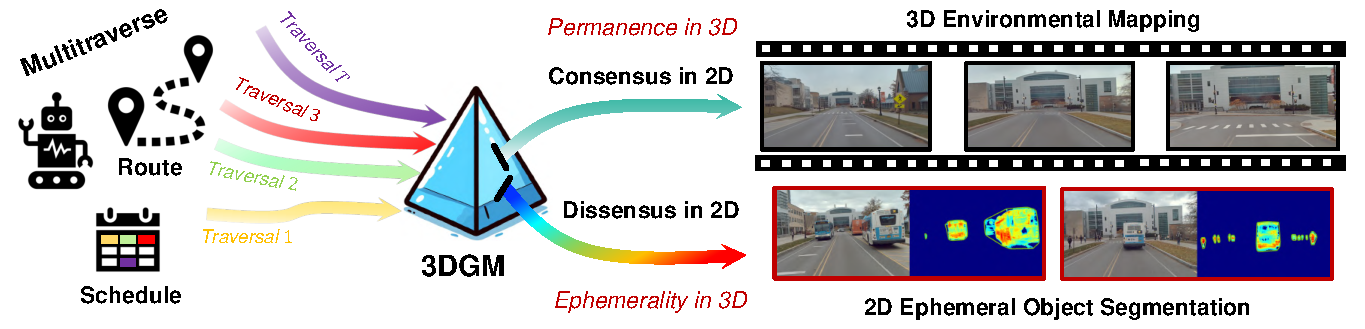
\includegraphics[width=\columnwidth]{figs_compressed/teaser_compressed.pdf}}
\caption{\textbf{A high-level diagram of \texttt{3D Gaussian Mapping (3DGM)}.} Given multitraverse RGB videos, \texttt{3DGM} outputs a Gaussian-based environment map (\texttt{EnvGS}) and 2D ephemerality segmentation (\texttt{EmerSeg}) for the input images. Note that the proposed framework is LiDAR-free and self-supervised. }
\label{fig:teaser}
\end{center}
\vspace{-7mm}
\end{figure}

\begin{quote}
\textit{Is it possible to develop an autonomous mapping system that can identify and memorize only the consistent environmental structures of the 3D world across multiple traversals, without relying on human supervision?}
\end{quote}

We provide an affirmative answer to this question. Our key insight is using the consensus across repeated traversals as the self-supervision signal, ensuring that the learned map retains only consensus structures (\textit{permanent environment}) while forgetting dissensus elements (\textit{transient objects}). We ground our insight in 3D Gaussian Splatting (3DGS)\cite{kerbl20233d}, which models a 3D scene using a group of 3D Gaussians with learnable attributes such as position, color, and opacity. This scene representation provides both geometric and photometric information, benefiting various downstream applications in autonomous driving. We utilize abundant images from multiple traversals to facilitate Gaussian initialization with Structure from Motion (SfM)~\cite{schonberger2016structure}, without using LiDARs. Subsequently, we learn the environmental Gaussians from multitraverse RGB videos by optimizing over the 2D image space.

To optimize a consistent 3D representation from input images with time-varying structures, we treat \textit{multitraverse environmental mapping} as a \textit{robust differentiable rendering} problem where pixels from transient objects are considered outliers. More specifically, we distill self-supervised robust features, denoised DINOv2~\cite{yang2024denoising,oquab2023dinov2}, into Gaussians to facilitate outlier identification. Afterward, we use a novel feature residual mining strategy to fully exploit the spatial information within the rendering loss map. This strategy aids in precise outlier grouping, enhancing transient object segmentation. Finally, we apply a robust loss function to optimize the 3D environmental Gaussians. Consequently, we can accurately learn the Gaussian-based environment map from inlier pixels and even generate 2D masks of transient objects for free, as illustrated in Fig.~\ref{fig:teaser}.

We build the \textit{\textbf{Map}ping and segmentation through multitra\textbf{verse}} (\textbf{Mapverse}) benchmark, sourced from the Ithaca365~\cite{diaz2022ithaca365} and nuPlan~\cite{karnchanachari2024towards} datasets to evaluate our method in three tasks: unsupervised 2D segmentation, 3D reconstruction, and neural rendering. Quantitative and qualitative results demonstrate the effectiveness of our method in autonomous driving scenarios. 

To summarize, our key innovations are listed as follows.
\begin{itemize}[leftmargin=1.3em]
    \item \textbf{{Problem formulation}}\quad We address the multitraverse RGB mapping problem through robust differentiable rendering, treating pixels of the environment as inliers and objects as outliers.

    \item \textbf{{Technical design}}\quad We introduce feature residuals mining to leverage spatial information from rendering loss maps, enabling more accurate outlier segmentation in self-driving scenes.

    \item \textbf{{System integration}}\quad We build 3D Gaussian Mapping (\texttt{3DGM}) that jointly generates 3D environmental Gaussians and 2D ephemerality masks without LiDARs and human supervision.

    \item \textbf{{Dataset curation}}\quad We build a large-scale multitraverse driving benchmark from real-world datasets for the community, featuring 40 locations, each with no less than 10 traversals, totaling 467 driving video clips and 35,304 images. This dataset will be released for further research.

\end{itemize}